Following~\cite{rah:vee:bir}, we use a Lagrangian formulation in which
we track the position of material points on $\gamma$ using multistep
implicit-explicit (IMEX) methods~\cite{ascher1995} to
discretize~\eqref{e:ves:dyn} in time. We use Nystr\"{o}m-type
quadrature rules to discretize integral operators and Fourier
differentiation to compute derivatives with respect to the membrane
parametrization.

\subsection{Spatial Discretization\label{s:spaceDisc}} 
Let $\xx(\alpha),$ with $\alpha \in (0,2\pi]$, be a parametrization of
the interface $\gamma_p$, $\{\alpha_k = 2k\pi/n\}_{k=1}^n$ be $n$
material points, and
\begin{align*}
  \xx(\alpha) = \sum_{k = -n/2+1}^{n/2} \hat{\xx}(k) e^{ik\alpha}.
\end{align*}
Using the FFT to compute $\hat{\xx}$, we compute derivatives of $\xx$
with spectral accuracy, assuming that $\gamma$ belongs to $C^{\infty}$.
In particular, we can compute the arclength derivative with spectral
accuracy since 
\begin{align*}
  \pderiv{}{s} = \pderiv{\alpha}{s}\pderiv{}{\alpha} = 
    \frac{1}{\|\partial\xx/\partial\alpha\|}\pderiv{}{\alpha},
\end{align*}
where $s$ is the arclength parametrization.

Since the single-layer potential $\SS$ has a logarithmic singularity, we
use the hybrid Gauss-trapezoid quadrature rule given in Table 8 of
\cite{alpert1999}.  The error of this quadrature rule is $\bigO(h^{8}
\log h)$ for integrands with logarithmic singularities. Letting $\xx_k =
\xx(\alpha_k)$, the quadrature rule is
\begin{align*}
  \mathcal S[\ff](\xx) \approx \sum_{k=1}^{n+m} w_{k}
      S(\xx,\xx_{k}) \ff(\xx_{k})\| \xx_{\alpha,k}\|,
\end{align*}
where $n$ is the number of nodes, $m$ is a number of additional
quadrature nodes, $w_{k}$ are the quadrature weights, $\xx_{k}$ are the
quadrature abscissae, and $\xx_{\alpha}$ is $\partial \xx/\partial
\alpha$.  The first $n$ abscissae are the usual equispaced quadrature
points.  Then, the other $m$, which is determined by the desired order
of convergence for the integral, are additional quadrature abscissas
clustered around the singularity.

The double-layer potential has no singularity in two dimensions since
\begin{align*}
  \lim_{\substack{\xx' \to \xx \\ \xx' \in \gamma}} D(\xx',\xx) = 
    \frac{\kappa(\xx)}{2\pi}({\bf t}(\xx) \otimes {\bf t}(\xx)),
  \quad \xx \in \gamma,
\end{align*}
where $\kappa$ is the curvature and ${\bf t}$ is the unit tangent.
Thus, a composite trapezoid rule will give spectral accuracy since the
integrand is periodic and smooth.


\subsection{Time discretization}
Time derivatives are discretized as
\begin{align*}
  \frac{d\xx}{dt} \approx \frac{\beta\xx^{N+1} - \xx^{0}}{\Delta t},
\end{align*}
where $\xx^{0}$ is a linear combination of previous time steps.
Operators and terms that are treated explicitly are discretized at
$\xx^{e}$ which is also a linear combination of previous time steps.
The simplest IMEX method is IMEX Euler which is given by $\beta=1$,
$\xx^{0} = \xx^{N}$, and $\xx^{e} = \xx^{N}.$ The second-order time
integrator we use is given by $\beta=3/2,$
\begin{align*}
\xx^{0} = 2\xx^{N} - \frac{1}{2}\xx^{N-1}, \hspace{20pt}
\xx^{e} = 2\xx^{N} - \xx^{N-1}.
\end{align*}
To avoid significant time stepping constraints, we treat the bending
term $\ff_{b}$ and tension term $\ff_{\sigma}$ semi-implicitly.  An
approximation for the position and tension of vesicle $p$ at time $N+1$
satisfies
\begin{subequations}
  \begin{align}
    \frac{\alpha_{p}}{\Delta t}(\beta \xx_{p}^{N+1} - \xx_{p}^{0}) &= 
      \SS_{p}^{e} \ff_{p}^{N+1} + 
      \DD_{p}^{e}\uu_{p}^{N+1} + \BB_{p}[\eeta^{N}] 
      + \sum_{\substack{q=1 \\ q \neq p}}^{M} \EE_{pq}^{e}[\ff_{q}^{N},\uu_{q}^{N}], 
      &&\xx \in \gamma_{p},
      \label{e:vesicle:dynamic:exp} \\
      \beta \mathcal{P}^{e}\xx_{p}^{N+1} &= \mathcal{P}^{e}\xx_{p}^{0},
      &&\xx \in \gamma_{p},
      \label{e:inextensibility:exp} \\
      U(\xx) &= -\frac{1}{2}\eeta^{N}(\xx) + \EE_{\Gamma}^{e}[\ff^{N},\uu^{N}](\xx) + 
      \BB[\eeta^{N}](\xx) + \mathcal{N}_{0}[\eeta^{N}](\xx), &&\xx \in \Gamma, 
      \label{e:BIE:exp} \\
      \uu_{p}^{N+1} &= \frac{\beta \xx_{p}^{N+1}-\xx_{p}^{0}}{\Delta t},
      &&\xx \in \gamma_{p},
      \label{e:velocity:exp}
  \end{align}
  \label{e:explicit:method}
\end{subequations}
where $\alpha_{p} = (1+\nu_{p})/2$, and operators with a superscript $e$
are discretized at $\xx^{e}$.  Note that~\eqref{e:explicit:method} has
explicit vesicle-vesicle and vesicle-boundary interactions.  That is, we
are approximating the solution of~\eqref{e:ves:dyn} with the solution of
a problem where the vesicles are fully decoupled from one another and
from the boundary.  To solve~\eqref{e:explicit:method}, we first find
$\eeta^{N}$ by solving~\eqref{e:BIE:exp} and then
solve~\eqref{e:vesicle:dynamic:exp} and~\eqref{e:inextensibility:exp}
for the new position and tension of each vesicle independently of all
the others.

In high-concentration flows, a new source of stiffness arises.  As two
vesicles approach one another, $\EE_{pq}$ becomes increasingly large.
A similar result holds for vesicle-boundary interactions where
$\BB_{p}$ introduces stiffness.  We propose the new method with
semi-implicit vesicle-vesicle and vesicle-boundary interactions (the
differences with \eqref{e:explicit:method} being highlighted in red)
\begin{subequations}
  \begin{align}
    \frac{\alpha_{p}}{\Delta t}
    (\beta \xx_{p}^{N+1} - \xx_{p}^{0}) &= 
      \SS_{p}^{e} \ff_{p}^{N+1} + \DD_{p}^{e}\uu_{p}^{N+1} + 
      \BB_{p}[\eeta^{N\textcolor{red}{+1}}] + \sum_{\substack{q=1 \\ q \neq p}}^{M} 
      \EE_{pq}^{e}[\ff_{q}^{N\textcolor{red}{+1}},
      \uu_{q}^{N\textcolor{red}{+1}}],
      &&\xx \in \gamma_{p},
      \label{e:vesicle:dynamic:imp} \\
      \beta \mathcal{P}^{e}\xx_{p}^{N+1} &= \mathcal{P}^{e}\xx_{p}^{0},
      &&\xx \in \gamma_{p},
      \label{e:inextensibility:imp} \\
      U(\xx) &= -\frac{1}{2}\eeta^{N\textcolor{red}{+1}}(\xx) + 
      \EE_{\Gamma}^{e}[\ff^{N\textcolor{red}{+1}},
      \uu^{N\textcolor{red}{+1}}](\xx) + 
      \BB[\eeta^{N\textcolor{red}{+1}}](\xx)+\mathcal{N}_{0}[\eeta^{N\textcolor{red}{+1}}](\xx), &&\xx \in \Gamma, 
      \label{e:BIE:imp} \\
      \uu_{p}^{N+1} &= \frac{\beta \xx_{p}^{N+1}-\xx_{p}^{0}}{\Delta t},
      &&\xx \in \gamma_{p}.
      \label{e:velocity:imp}
  \end{align}
  \label{e:implicit:method}
\end{subequations}
Unlike in~\eqref{e:explicit:method}, vesicles
in~\eqref{e:implicit:method} are implicitly coupled since the operator
$\EE_{pq}^{e}$ is applied to $\ff_{q}^{N+1}$ and $\uu_{q}^{N+1}$.
Similarly, the operator $\BB_{p}$ implicitly couples the vesicles to the
solid walls.  Equation~\eqref{e:implicit:method} is still an
approximation of~\eqref{e:ves:dyn}, but its benefit is that it is
experimentally a more stable method (see Sections~\ref{s:taylorGreen}
and~\ref{s:couette}).

Since~\eqref{e:implicit:method} is fully coupled, it is too expensive to
solve without preconditioning.  Roughly speaking, the number of GMRES
iterations depends on the sizes of $\EE_{pp}$ and $\EE_{pq}$ and the
latter depends on the inter-vesicle proximity.  We apply preconditioned
GMRES~\cite{saad} to~\eqref{e:implicit:method} where we use the
block-diagonal preconditioner.  The number of GMRES iterations depends
on the minimum inter-vesicle distance, but this preconditioned linear
system experimentally results in mesh-independence\footnote{We
experimented with multigrid preconditioners~\cite{quaife:biros2013} but
mesh-independence was only achieved for computationally expensive
preconditioners.}.

To test the preconditioner, one step of a Taylor-Green flow is done
with the number of points per vesicle ranging from $16$ to $128$
(Table~\ref{t:GMRES:preco}).  We solve~\eqref{e:implicit:method} to a
tolerance of $10^{-8}$ with and without preconditioning.  The required
GMRES iterations for the block-diagonal solver grows almost linearly
and the results are consistent with those reported
in~\cite{rah:vee:bir}.  The implicit solver without preconditioning
requires an unacceptable number of GMRES iterations, but with
preconditioning, we see that the required number of GMRES steps is
independent of $N$ \footnote{Notice, however, that the number of GMRES
iterations will depend on how close the vesicles are to one another as
this determines the overall spectrum structure of the operator. But for
a given flow, the method is independent of $N$.}.  Using the
block-diagonal preconditioner will not result in a speedup unless we
precompute and store the block diagonal preconditioner.  We perform
this precomputation for all the experiments in Section~\ref{s:results}.

\begin{table}[htp]
\centering
\begin{tabular}{>{\centering}m{0.5cm} >{\centering}m{3cm} >{\centering}m{3cm} >{\centering}m{3cm}}
$N$ & Block- \\ Diagonal & Unpreconditioned \\ Implicit & Preconditioned
\\ Implicit \tabularnewline
\hline
16 & 46 & 315 & 18 \tabularnewline
32 & 79 & 341 & 15 \tabularnewline
64 & 164 & 882 & 15 \tabularnewline
128 & 294 & 2117 & 15 
\end{tabular}
\mcaption{The number of GMRES iterations required to take one time step
of a Taylor-Green flow using semi-implicit inter-vesicle
interactions~\eqref{e:implicit:method}.  $N$ is the number of
discretization points per vesicle, the second column is the number of
GMRES iterations to invert the block-diagonal preconditioner, the third
column is the number of unpreconditioned GMRES iterations, and the
final column is the number of preconditioned GMRES iterations.  Notice
that without preconditioning, the number of iterations quickly grows
while the preconditioned linear system is
mesh-independent.}{t:GMRES:preco}
\end{table}
We have also observed experimentally that when vesicles are close,
treating inter-vesicle interactions explicitly with second-order time
stepping is unconditionally unstable.  We have experimented with time
step sizes of varying orders of magnitude and each experiment
inevitably becomes unstable.  However, scheme~\eqref{e:implicit:method}
with second-order time stepping is stable once $\Delta t$ is small
enough for the simulation under consideration.

\subsection{Fast summation}
For high-concentration flows, the most expensive part of the simulation
is evaluating the integral operators $\SS$ and $\DD$.  The single-layer
potential $\SS$ can be written as
\begin{align*}
  \frac{1}{4\pi\mu_{0}} \int_{\gamma}  \left(
    -\boldsymbol{I}\log \rho  + 
    \frac{\rr \otimes \rr}{\rho^{2}} \right)\ff ds = 
    -\frac{1}{4\pi\mu_{0}} \int_{\gamma} (\log \rho) \ff ds +
    \frac{1}{4\pi\mu_{0}} \int_{\gamma}
    \left(\frac{\rr \cdot \ff}{\rho^{2}}\right)\rr ds \\
  =-\frac{1}{4\pi\mu_{0}} \int_{\gamma}(\log \rho) \ff ds + 
    \frac{1}{4\pi\mu_{0}} \int_{\gamma}   
    \frac{\rr}{\rho^{2}} (\xx \cdot \ff) ds_{\yy} - 
    \frac{1}{4\pi\mu_{0}} \int_{\gamma} 
    \frac{\rr}{\rho^{2}} (\yy \cdot \ff) ds_{\yy},
\end{align*}
which can be computed with three Laplace FMM applications.  We also use
the FMM to evaluate the single-layer potential at arbitrary target
locations by assigning a charge of zero to these locations.
Unfortunately, the double-layer potential can not be decomposed into a
sequence of Laplace single- and double-layer potentials.  Future work
involves using the kernel-independent FMM~\cite{ying-biros-zorin-03} to
accelerate evaluating the double-layer potential.


\subsection{Near-singular integration}\label{s:near-singular}
Another difficulty with high-concentration simulations is the
evaluation of layer potentials at points close to a boundary.  Integral
operators $\DD$ and $\SS$ can be approximated with high accuracy using
the trapezoid rule if the target point is sufficiently far from the
source points.  As the target point approaches the vesicle,
more points are required to achieve the same accuracy, and, the
required number of points for a fixed error grows without
bound (Appendix~\ref{A:AppendixA}).  A near-singular integration
strategy that guarantees a uniform accuracy for all target points is
required.  

We adopt the strategy from~\cite{ying-biros-zorin06} since it is not
depend on the nature of the integrand and it is simple to implement.
Suppose that a vesicle $\gamma$ is discretized with $N$ points and that
the resulting arclength term is of size $h$.  Let $d(\xx,\gamma) =
\inf_{\yy \in \gamma} \|\xx - \yy\|$ be the distance from $\xx$ to
$\gamma$.  We define the far zone of $\gamma$ as $\Omega_{1}=\{\xx
\:|\: d(\xx,\gamma) \geq h\}$, and the near zone of $\gamma$ as
$\Omega_{0}=\{\xx \:|\: d(\xx,\gamma) < h\}.$ The near and far zones
can be constructed efficiently using a quadtree-structure, similar to
the near-field and far-field interactions in fast multipole codes.

For $\xx \in \Omega_{1}$, the trapezoid rule with $N^{3/2}$ points
guarantees that the error for $\SS$ is $\mathcal{O}(h^{M/2-2})$ and for
$\DD$ is $\mathcal{O}(h^{M/2-4})$, where the density function (in our
case, either $\ff$ or $\eeta$) belongs to $C^{M}$.  These error bounds
are proved in Appendix~\ref{A:AppendixA}.  For a target point $\xx$ in
the near zone, we first find the closest boundary point, $\xx_{0}$,
using two applications of Newton's method with the initial guess being
the closest discretization point to $\xx$.  We then place $m$
interpolation points at the points $\xx_{j} = \xx_{0} + j\beta h
(\xx-\xx_{0})/\|\xx-\xx_{0}\|$ for $j=0,\ldots,m$, where $\beta$ is
slightly larger than $1$ to guarantee that all the interpolation points
are in the far zone (left plot of Figure~\ref{f:nearsing:conv}).  The
layer potential is evaluated at $\xx_{0}$ using a local interpolant with
$N_{\mathrm{int}}$ points on $\gamma$ and evaluated at $\xx_{j},$
$j=1,\ldots,m$ using the $N^{3/2}$-point trapezoid rule.  Then, a
one-dimensional Lagrange interpolation assigns a value to the layer
potential at $\xx$.  Note that the proposed scheme can become more
accurate by using interpolation schemes that compute derivatives of the
solution and building more accurate polynomial interpolations.  This,
however, would significantly complicate the implementation.  Pseudocode
for this algorithm is given in Algorithm~\ref{a:algorithm2}.  In
Appendix~\ref{A:AppendixA}, we show that the error of our algorithm
applied to the single-layer potential $\SS$ is 
\begin{align*}
  \bigO\left(h^{\min\left(N_{\mathrm{int}}-1,
      m,\frac{M}{2}-2\right)}\right),
\end{align*}
and applied to the double-layer potential $\DD$ is
\begin{align*}
  \bigO\left(h^{\min\left(N_{\mathrm{int}}-1,
      m,\frac{M}{2}-4\right)}\right).
\end{align*}

\begin{algorithm}
\begin{algorithmic} 
\FORALL[Loop over far zone]{$\xx \in \Omega_{1}$} 
\STATE $\uu = \mathtt{trapezoid}(\gamma,\xx,\ff)$
\COMMENT{Apply the $N^{3/2}$-point trapezoid rule}
\ENDFOR 
\FORALL[Loop over near zone]{$\xx \in \Omega_{0}$}
\STATE $\xx_{0} = \argmin d(\xx,\gamma)$
\COMMENT{Find the point on $\gamma$ closest to $\xx$}
\STATE $\uu_{0} = \mathtt{interpolate}
    (\xx_{0},\uu_{1},\ldots,\uu_{N_{\mathrm{int}}})$
\COMMENT{Interpolate $\uu$ at $\xx_{0}$}
\FOR{$j=1,\ldots,m$}
\STATE $\xx_{j} = \xx_{0} + jh\beta(\xx-\xx_{0})/\|\xx-\xx_{0}\|$
\COMMENT{Define Lagrange interpolation points}
\STATE $\uu_{j} = \mathtt{trapezoid}(\gamma,\xx_{j},\ff)$
\COMMENT{Evaluate layer potential at $\xx_{j}$}
\ENDFOR 
\STATE $\uu = \mathtt{interpolate}(\xx,\uu_{0},\ldots,\uu_{m})$
\COMMENT{Compute $\uu$ using Lagrange interpolation}
\ENDFOR 
\RETURN $\uu$ \COMMENT{Return the layer potential at all target points}
\end{algorithmic}
\mcaption{LayerPotential($\gamma$,  $\ff$, $\uu$, $\Omega_{0}$,
$\Omega_{1}$)} {a:algorithm2}
\end{algorithm}

\begin{figure}[htp]
  \begin{center}
    \begin{minipage}{0.45\textwidth}
    \input{figs/near-sing.tikz}
    \end{minipage}
    \begin{minipage}{0.45\textwidth}
    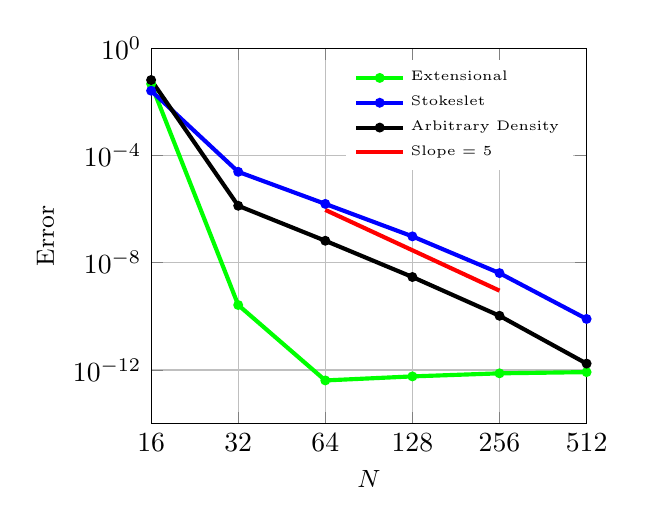
\begin{tikzpicture}[scale=1]

\begin{axis}[
  width=2.8in, height=2.5in,
  xmin = 16,
  xmax = 512,
  ymin = 1e-14,
  ymax = 1e0,
  xlabel = {$N$},
  ylabel = {Error},
  xtick = {16,32,64,128,256,512},
  xticklabels = {$16$,$32$,$64$,$128$,$256$,$512$},
  ytick = {1e-12,1e-8,1e-4,1e0},
  yticklabels = {$10^{-12}$,$10^{-8}$,$10^{-4}$,$10^{0}$},
  label style = {font=\small},
  xmode = log,
  ymode = log,
  grid,
  legend entries = {Extensional,Stokeslet,Arbitrary Density,Slope = 5},
  legend pos = north east,
  legend style = {draw=none,font=\tiny},
  legend cell align = left 
  ]

\addplot [mark=*,mark size=1pt,green,line width=1.5] table{
16 4.66e-2
32 2.65e-10
64 4.08e-13
128 5.77e-13
256 7.51e-13
512 8.34e-13
};

\addplot [mark=*,mark size=1pt,blue,line width=1.5] table{
16 2.59e-2
32 2.45e-5
64 1.56e-6
128 9.60e-8
256 4.10e-9
512 8.01e-11
};

\addplot [mark=*,mark size=1pt,black,line width=1.5] table{
16 6.50e-2
32 1.33e-6
64 6.59e-8
128 2.93e-9
256 1.05e-10
512 1.73e-12
};

\addplot [mark=none,red,line width=1.5] table{
%16 9.5367e-4
%32 2.9802e-5
64 9.3132e-7
128 2.9104e-8
256 9.0949e-10
%512 2.8422e-11
};

\end{axis}

%\draw[gray,thin] (0,0) grid +(3,4);

\end{tikzpicture}

 
    \end{minipage} 
  \end{center} 
  \mcaption{\emph{Left:} Lagrange interpolation points in $\Omega_{1}$
  and $\gamma$ are used to approximate layer potentials at $\xx \in
  \Omega_{0}$.  The value at $\xx_{0}$ uses an interpolant from
  neighboring points on the boundary.  All other interpolation points
  are in $\Omega_{1}$ so that the $N^{3/2}$-point trapezoid rule is
  sufficiently accurate.  \emph{Right:} Here we report convergence
  rates. For the blue and the black curves, the expected order of
  convergence is $5$. We obtain $4.7$ and $5.0$, respectively. As the
  green curve corresponds to a linear flow, Lagrange interpolation gives
  exact values.  Hence, machine accuracy is reached once $N$ is
  sufficiently large.}{f:nearsing:conv}
\end{figure}

We test our near-singular integration with three examples.  In all the
examples, 32 target points are placed in $\Omega_{0}$ for
$N=16,\ldots,512$.  The boundary is a $3:2$ ellipse, the boundary values
are interpolated with $N_{\mathrm{int}}=6$ points, and the Lagrange
interpolation uses $m=6$ points.  Since $m = N_{\mathrm{int}}$, we are
using one more point to interpolate in the direction coming off of
$\gamma$.  We do this because the interpolant that is coming off of the
vesicle is always evaluated near the first interpolation point.  Thus,
it may suffer from the Runge phenomenon (we have observed this
experimentally).  This is not the case for the local interpolation used
to find $\uu(\xx_{0})$ since $\xx_{0}$ is located near the middle of the
local interpolation points.  For the first two examples, we compute the
density function of $\SS$ for the two solutions of the Stokes equations:
\begin{align*}
  &\uu(\xx)=(x,-y), \\
  &\uu(\xx)=\left(-\log|\xx| + \frac{\xx \otimes \xx}{|\xx|^{2}}\right)
  \left[ \begin{array}{c}
    1 \\ 1 
  \end{array}\right].
\end{align*}
For the third example, we pick an arbitrary density function and compare
the results from near-singular integration with the results from an
over-refined trapezoid rule.  The error for all three examples is
reported in~Figure~\ref{f:nearsing:conv}.  For the extensional flow $\uu
= (x,-y)$, the Lagrange interpolation is exact since the flow is linear
and the error decays faster than the other examples.  For the other
examples, the error is close to fifth-order which agrees with the order
of accuracy of the near-singular integration

If we have $M$ vesicles and $N$ points per vesicle, the major costs of
the near-singular integration algorithm are:
\begin{itemize}
  \item \emph{Upsampling each vesicle from $N$ to $N^{3/2}$ points:}
  Using the FFT, this requires $\bigO(MN^{3/2}\log N)$ operations.
  \item \emph{Applying the $N^{3/2}$-point quadrature rule to
  $\Omega_{1}$:} With the FMM, this requires $\bigO(MN^{3/2} + MN)$
  operations, and without the FMM, this requires $\bigO(M^{2}N^{5/2})$
  operations.  
  \item \emph{Evaluating the layer potential in $\Omega_{0}$:} Assuming
  there are $\bigO(1)$ points in the near zone, this requires
  $\bigO(MN^{3/2})$ operations.
\end{itemize}
The algorithm can be further sped up by introducing the intermediate and
far zones~\cite{ying-biros-zorin06}.  The intermediate zone is
$\Omega_{1}=\{\xx \:|\: d(\xx,\gamma) \in (\sqrt{h},h]\}$ and the far
zone is $\Omega_{2}=\{\xx \:|\: d(\xx,\gamma) \geq \sqrt{h}\}$.  Then,
the same accuracy can be achieved by using the $N^{3/2}$-point trapezoid
rule in $\Omega_{1}$ and the $N$-point trapezoid rule in $\Omega_{2}$.
While this would reduce the constant of the complexity, it does not
change the overall order and complicates the implementation.


\subsection{Collision detection}\label{s:collision}
Even with semi-implicit treatment of inter-vesicle interactions, due
to time discretization errors, the vesicles can come so close that they
collide or cross a solid wall.\footnote{The streamlines of Stokes
equations never intersect.  Therefore, it is physically impossible for
vesicles to collide with one another or with solid walls in finite
time.  Lubrication theory can be used to study the forces between
nearly touching vesicles, and therefore compute estimates of the
distance between the vesicles, but we choose not to discuss these
forces here.}  There has been a lot of work in collision
detection~\cite{jimenez-e13,redon-e04}, but they are not spectrally
accurate or require complex surface-surface intersections.  Most
methods construct piecewise approximations to the boundaries to
simplify the detection of collisions.  Since our vesicles and solid
walls are periodic, we can use some nice properties of layer potentials
to create a spectrally accurate collision detector.  We use the classic
potential theory result~\cite{kellogg}
\begin{align}
  I_{\Gamma}(\xx) = \frac{1}{2\pi}\int_{\Gamma}\pderiv{}{\nn_{\yy}}\log|\xx - \yy| ds_{\yy} = 
  \begin{cases}
    1 & \xx \in \Omega, \\ 
    \frac{1}{2} & \xx \in \Gamma, \\ 
    0 & \xx \in \mathbf{R}^{2} \backslash \overline{\Omega}, 
  \end{cases}
  \label{e:layerpotentials}
\end{align}
where $\Omega \subset \mathbf{R}^{2}$ is bounded with a smooth boundary
$\Gamma$, and $\nn_{\yy}$ is the outward pointing normal.  We
apply~\eqref{e:layerpotentials} to the configuration of the vesicles
and the solid walls by computing $I_{X}(\xx) = I_{\gamma_{1}}(\xx) +
\cdots + I_{\gamma_{M}} + I_{\Gamma}$ for all $\xx \in \gamma$.  The
maximum value of $I_{X}(\xx)$ is $3/2$ for confined flows and $1/2$ for
unconfined flows if vesicles have not crossed and have not left the
domain.  The maximum value of $I_{X}(\xx)$ will be at least $3/2$ for
unconfined flows, and at least $5/2$ for confined flows if vesicles
have crossed or left the domain.  We note that $I_{X}(\xx)$ can be
evaluated accurately using our near-singular integration scheme, and in
linear time using the FMM. 

We can use $I_{X}(\xx)$ to create a simple adaptive time-stepping
method.  At each time step, we check for collisions.  If a collision has
occurred, we initialize the simulation at a previous time step with a
time step half the size.  We are currently implementing a more rigorous
adaptive time stepping method that uses ideas from spectral deferred
correction methods~\cite{dut:gre:rok,hua:jia:min,min}.  At each time
step, we estimate the local truncation error and then try to commit a
constant amount of error per time step by adjusting the time step size.
We leave the details and the implementation as future work.  Future work
also includes adaptivity in space.  If vesicles are sufficiently far
from one another, their hydrodynamic interaction can be represented with
a moderate number of points, but as they approach one another, the
hydrodynamic interaction strengthens and this requires a finer spatial
resolution.

